\chapter{向量与线性代数：二维箭头通向高维空间}

前面几章里，我们学会了用字母搬运数、用方程研究关系、用坐标把代数和几何缝在一起，还看过平移、旋转、翻折这些“动作”怎样组成对称的家族。这一章我们要做一件看起来很小、实际上改变整个数学面貌的事：给平面上的每一个“移动”画一支箭头，然后问——这些箭头本身能不能像数一样相加、相乘、被研究？

答案不但能，而且一旦做到这一点，二维的游戏画面、三维的动画、几万维的网页排序、甚至琴弦的振动，全都变成了同一套语言的练习题。这套语言叫线性代数。它是现代数学里应用最广的分支之一，而它的起点，只是平面上的一支箭头。

\section{游戏里的一个下午}

想象你在玩一款俯视角的冒险游戏。你的角色站在一片草原上，屏幕上没有东西南北，只有角色自己的朝向。键盘上有两个键：一个让角色“向前跨一步”，一个让角色“向左横移一步”。

下午的任务是走到地图上的一口井。你面朝东北方向，先向前跨了 $3$ 步，又向左横移了 $2$ 步，发现走过头了，于是掉头向前跨了 $1$ 步。问题来了：折腾这一通之后，你离出发点到底多远？方向朝哪？

如果只是问“你一共走了几步”，小学生都会算：$3+2+1=6$ 步。但你真正想问的显然不是这个——走 $6$ 步可能绕回原地，也可能走出老远。你想问的是：从出发点到终点，那支“可以直接飞过去”的箭头长什么样？

这个游戏里的困惑每天都在真实世界重演。快递员先向东骑 $3$ 公里，又向北骑 $4$ 公里，他离站点多远？帆船先被风吹向东南，又被洋流推向东北，最终漂到了哪里？无人机同时收到“上升”和“前进”两个指令，它的实际航线是什么？这些问题都有一个共同结构：几次移动叠在一起，要合成一次总的移动。

先凭直觉猜一猜：向东 $3$ 公里再向北 $4$ 公里，离出发点多远？很多人第一反应是 $7$ 公里。也有人隐约记得勾股定理，猜 $5$ 公里。哪个对？更重要的是：我们能不能发明一套记法，让这一类问题永远不用重新猜？

\section{第一次尝试：只记数字够吗}

最自然的尝试是：把每次移动记成一个数——走了多远。然后把数加起来。

这个方案立刻会撞上灾难。假设快递员向东骑了 $3$ 公里，掉头又向西骑了 $3$ 公里。按“路程”记账，他奔波了 $6$ 公里，汗水是真的；可按“离站多远”记账，他就在站点门口，等于哪儿也没去。两笔一模一样的“$3$ 公里”，叠在一起的结果却是零。

\begin{fanli}
有人说：“两次移动合起来，总移动的距离就是两次距离相加。”这对吗？找一个反例：向东走 $3$ 公里，再向西走 $3$ 公里。$3+3=6$，但人回到了原地，总位移是 $0$。错误出在哪？出在“距离”这个数里根本不包含方向的信息。两个方向相反的移动，在距离账本上长得一模一样，在真实世界里却互相抵消。任何试图用一个数描述移动的方案，都会在这类反例上翻车。
\end{fanli}

失败给了我们一条重要线索：移动这种东西，天生带着两样信息——走了多远，以及朝哪个方向。丢掉方向，数字再大也没法相加出正确答案。我们需要的新概念必须同时装下这两样信息。

还有一个更隐蔽的麻烦。就算我们记下“向东 $3$ 公里”“向北 $4$ 公里”这样的短语，叠加三次、五次之后，口头描述会变成一团乱麻：“先向东再向北再向东南再向西北……”我们需要的是一套能算的记法——像数一样可以相加、可以乘倍、可以列式子，而不是一篇游记。

\section{发明箭头：向量的诞生}

解决方案朴素得让人意外：既然移动有方向有距离，那就干脆画一支箭头来代表它。箭头的指向就是移动的方向，箭头的长度就是移动的距离。

\begin{shuyu}{向量}
直观解释：一支有方向、有长度的箭头，代表一次移动、一个力、一个速度——任何“大小加方向”的量。

正式定义：平面（或空间）中由一对（或一组）有序实数确定的对象，记作 $\vec{v}=(x,y)$。两个向量相等，当且仅当它们方向相同、长度相等，与画在哪里无关。

例子：从原点指向点 $(3,4)$ 的箭头是向量 $(3,4)$，它的长度是 $\sqrt{3^2+4^2}=5$。
\end{shuyu}

注意定义里那句“与画在哪里无关”。向东 $3$ 公里这支箭，从你家门口画和从学校门口画，是同一个向量。向量只记录“怎么动”，不记录“站在哪”。这个约定初看奇怪，其实是向量好算的关键：它让我们可以把所有箭头平移到同一个起点来比较。

向量的伟大之处在于，它的加法是被几何逼出来的，而不是被规定出来的。先走 $\vec{a}$ 再走 $\vec{b}$，总效果是什么？把 $\vec{b}$ 的尾巴接到 $\vec{a}$ 的箭尖上，从起点画到终点的那支箭就是答案，记作 $\vec{a}+\vec{b}$。这就是著名的三角形法则；换一种画法，把两支箭尾巴对齐、补成一个平行四边形，对角线就是和。

\begin{center}
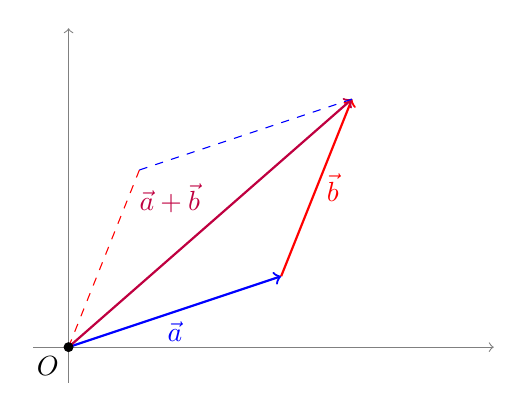
\begin{tikzpicture}[scale=0.9]
  \draw[->,gray] (-0.5,0) -- (6,0);
  \draw[->,gray] (0,-0.5) -- (0,4.5);
  \draw[->,thick,blue] (0,0) -- (3,1) node[midway,below] {$\vec{a}$};
  \draw[->,thick,red] (3,1) -- (4,3.5) node[midway,right] {$\vec{b}$};
  \draw[->,thick,purple] (0,0) -- (4,3.5) node[midway,above left] {$\vec{a}+\vec{b}$};
  \draw[dashed,red] (0,0) -- (1,2.5);
  \draw[dashed,blue] (1,2.5) -- (4,3.5);
  \fill (0,0) circle (2pt) node[below left] {$O$};
\end{tikzpicture}
\end{center}

用坐标来算，加法简单得不像话：对应分量分别相加。
\[
(3,1)+(1,2.5)=(3+1,\;1+2.5)=(4,3.5).
\]
几何上的“首尾相接”，代数上的“分量相加”，是同一件事的两种语言——这正是第 4 章那座坐标桥梁的又一次通车。

有了加法，自然有“加倍”：把一支箭拉长到原来的 $2$ 倍、缩短到一半、或者翻转方向，叫作数乘，记作 $2\vec{v}$、$\tfrac{1}{2}\vec{v}$、$-\vec{v}$。坐标上就是把每个分量乘以同一个数：$2\cdot(3,4)=(6,8)$。

现在回到游戏里的困惑。把“向前一步”记作向量 $\vec{f}$，“向左一步”记作向量 $\vec{l}$。你下午的全部行踪——向前 $3$ 步、向左 $2$ 步、掉头向前 $1$ 步——就可以写成一个式子：
\[
3\vec{f}+2\vec{l}+(-1)\vec{f}=2\vec{f}+2\vec{l}.
\]
游记压缩成了一行代数。像 $3\vec{f}+2\vec{l}$ 这样“若干向量各自乘上倍数再相加”的东西，叫做这些向量的\textbf{线性组合}。“线性”这个词的意思是：只允许做加法和数乘这两件最朴素的事，不允许向量互相乘、平方或者更花俏的操作。别小看这个限制——只允许两件朴素操作的数学，恰好是世界上最强大的数学之一。

接下来的问题决定了整章的走向：选哪几支箭当“基本步伐”，才能让平面上所有可能的移动都写成它们的线性组合？

一支箭显然不够：只会“向前”，你永远到不了侧方的井。两支不共线的箭呢？比如 $\vec{f}$ 朝东、$\vec{l}$ 朝北。直觉上，朝任何方向的移动都能拆成“先走多少东、再走多少北”。在平面上，两支不同方向的箭似乎就够用了；而第 $3$ 支箭（比如东北方向）是多余的，因为它本身已经是前两支的线性组合。

\begin{shuyu}{基与维数}
直观解释：基是一组“基本步伐”，少一个就走不全，多一个就有冗余；维数就是这组步伐的个数。

正式定义：如果一组向量线性无关（谁也不是其他成员的线性组合），并且它们的所有线性组合能铺满整个空间，就称这组向量为空间的一组基；基中向量的个数叫做空间的维数。

例子：平面上 $\vec{e}_1=(1,0)$ 与 $\vec{e}_2=(0,1)$ 是一组基，平面是二维的；$(1,0)$ 与 $(1,1)$ 也是一组基——基并不唯一。
\end{shuyu}

“维数”这个被我们随口用了十几年的词，在这里第一次有了精确的意思：一个空间是几维的，就是问它最少需要几个独立的“基本方向”才能拼出所有的向量。直线是一维的，平面是二维的，我们生活的空间是三维的——而代数对此毫不在意，$(x_1,x_2,\dots,x_{100})$ 这样的一百个分量排成一排，照样可以加、可以数乘，照样是一个一百维空间里的向量。箭头画不出来了，但算术照常运转。这就是标题里“通向高维空间”的含义：二维的直觉，通过代数规则，原封不动地搬运到了眼睛看不见的地方。

\section{核心定理：每个箭头只有一种写法}

凭什么相信“两支不同方向的箭就能拼出平面上的一切”？凭直觉不行，我们把它变成一个定理，并且证明它。

\begin{dingli}[坐标的唯一性]
设 $\vec{e}_1$ 和 $\vec{e}_2$ 是平面上两个不共线的向量。那么平面上任意一个向量 $\vec{v}$ 都可以唯一地写成
\[
\vec{v}=a\vec{e}_1+b\vec{e}_2,
\]
其中 $a$、$b$ 是实数。也就是说：表示一定存在，而且系数只有一组。
\end{dingli}

\begin{proof}
先证存在性。把 $\vec{e}_1$、$\vec{e}_2$ 和 $\vec{v}$ 的尾巴都平移到同一点 $O$。过 $\vec{v}$ 的箭尖，作一条平行于 $\vec{e}_2$ 的直线，它与 $\vec{e}_1$ 所在的直线相交于一点 $P$（因为 $\vec{e}_1$ 与 $\vec{e}_2$ 不共线，这两条直线不平行，必相交）。从 $O$ 到 $P$ 的箭头与 $\vec{e}_1$ 共线，所以它是 $\vec{e}_1$ 的某个倍数 $a\vec{e}_1$；从 $P$ 到 $\vec{v}$ 箭尖的那段与 $\vec{e}_2$ 共线，是某个倍数 $b\vec{e}_2$。由向量加法的三角形法则，$\vec{v}=a\vec{e}_1+b\vec{e}_2$。

再证唯一性。假设同一支箭有两种写法：
\[
\vec{v}=a\vec{e}_1+b\vec{e}_2=a'\vec{e}_1+b'\vec{e}_2.
\]
两式相减得 $(a-a')\vec{e}_1+(b-b')\vec{e}_2=\vec{0}$。如果 $a-a'\neq 0$，就能解出
\[
\vec{e}_1=-\frac{b-b'}{a-a'}\,\vec{e}_2,
\]
这说明 $\vec{e}_1$ 是 $\vec{e}_2$ 的倍数，即两箭共线，与假设矛盾。所以 $a=a'$，同理 $b=b'$。表示法只有一组。
\end{proof}

这个定理值得停下来端详一会儿。它说的是：一旦选定基，平面上每个向量就和一对有序实数 $(a,b)$ 一一对应。向量是几何对象，坐标是代数对象，这一定理保证了翻译是完美无损的——不多也不少。我们在第 4 章天天写坐标 $(x,y)$，其实一直在默认这个定理成立；现在它终于从后台走到台前，被正式证明了。

同一套“线性组合”的脑子，顺手就能解开第 2 章留下的一个几何谜团：二元一次方程组
\[
\begin{cases}
2x+y=5,\\
x-y=1
\end{cases}
\]
到底在画什么？有两种看法，都正确，都重要。

第一种看法是“一行一行看”：每个方程是一条直线，解就是两条直线的公共点。两条直线相交，恰有一个解；平行不重合，无解；重合，无穷多解。三种情况，再无其他——因为平面上两条直线的关系就只有这三种。数值验证一下：相加得 $3x=6$，即 $x=2$，代入得 $y=1$，交点是 $(2,1)$。

\begin{center}
\begin{tikzpicture}[scale=0.7]
  \draw[->,gray] (-1,0) -- (6,0) node[right] {$x$};
  \draw[->,gray] (0,-2) -- (0,5.5) node[above] {$y$};
  \draw[thick,blue] (-0.5,6) -- (3.5,-2) node[below right] {$2x+y=5$};
  \draw[thick,red] (0.5,-0.5) -- (5,4) node[above right] {$x-y=1$};
  \fill (2,1) circle (2.5pt) node[below right] {$(2,1)$};
\end{tikzpicture}
\end{center}

第二种看法是“一列一列看”，把方程组改写成
\[
x\begin{pmatrix}2\\1\end{pmatrix}+y\begin{pmatrix}1\\-1\end{pmatrix}=\begin{pmatrix}5\\1\end{pmatrix}.
\]
它问的是：用 $(2,1)$ 和 $(1,-1)$ 这两支箭，各取多少倍，才能拼出目标箭 $(5,1)$？方程组有唯一解，正因为这两支箭不共线——它们构成一组基，定理保证拼法恰有一种。无解的情况对应两支箭共线而目标箭不在这条线上：怎么拼都够不着。无穷多解对应三者都共线：拼法随便挑。

升到三维：每个三元一次方程是空间中的一个平面。三个平面可以交于一点（唯一解），交成一条线（无穷多解），或者像翻开的书页那样两两相交却没有公共点（无解）。代数里“方程组有没有解、有几个解”的问题，在几何里变成了“几个平面怎么摆放”的问题。线性代数这门学问，本质上就是把这两幅图景来回翻译的艺术。

\section{矩阵：把变换装进格子}

第 6 章我们研究过旋转、缩放、翻折这些“动作”。当时我们用几何语言描述它们：把整个平面绕原点转 $90^\circ$，把每点到原点的距离放大 $2$ 倍。现在有了向量和坐标，可以问一个更实用的问题：能不能给每种动作配一张“说明书”，让我把任意一点的坐标代进去，就能算出它动作之后的新坐标？

先看旋转 $90^\circ$（逆时针）。拿两支基箭做实验：$\vec{e}_1=(1,0)$ 转到了 $(0,1)$，$\vec{e}_2=(0,1)$ 转到了 $(-1,0)$。由坐标的唯一性，任意向量 $(x,y)=x\vec{e}_1+y\vec{e}_2$ 转完就是
\[
x\cdot(0,1)+y\cdot(-1,0)=(-y,\;x).
\]
拿一个具体点验证：$(3,1)$ 转完应该是 $(-1,3)$。在方格纸上画一下，确实如此——箭头长度没变，方向逆时针转了一个直角。

把两个基向量的像 $(0,1)$ 和 $(-1,0)$ 并排写成两列，装进一个方格子：
\[
A=\begin{pmatrix}0&-1\\1&0\end{pmatrix}.
\]
这个方格子叫矩阵。约定 $A$ 乘向量 $(x,y)$ 的规则是“行点乘列”：
\[
\begin{pmatrix}0&-1\\1&0\end{pmatrix}\begin{pmatrix}x\\y\end{pmatrix}
=\begin{pmatrix}0\cdot x+(-1)\cdot y\\1\cdot x+0\cdot y\end{pmatrix}
=\begin{pmatrix}-y\\x\end{pmatrix}.
\]
格子第一行算出结果的第一个分量，第二行算出第二个分量。整张平面的旋转，就这样被压缩进了四个数字。

再看缩放。把所有点到原点的距离放大 $2$ 倍，$\vec{e}_1$ 不动方向变长为 $(2,0)$，$\vec{e}_2$ 变成 $(0,2)$，矩阵是
\[
\begin{pmatrix}2&0\\0&2\end{pmatrix},
\]
它把 $(x,y)$ 变成 $(2x,2y)$。类似地，沿 $x$ 轴的翻折是 $\begin{pmatrix}1&0\\0&-1\end{pmatrix}$，水平方向的切变是 $\begin{pmatrix}1&1\\0&1\end{pmatrix}$。

为什么矩阵装得下这些变换？因为旋转、缩放、翻折、切变有一个共同的“好脾气”：它们把直线仍变成直线，把原点固定不动，并且满足
\[
T(\vec{u}+\vec{v})=T(\vec{u})+T(\vec{v}),\qquad T(c\vec{v})=c\,T(\vec{v}).
\]
具有这两条性质的变换叫\textbf{线性变换}。这两条的威力在于：只要知道变换把两支基箭送到哪里，任意向量 $x\vec{e}_1+y\vec{e}_2$ 的去向就被迫确定了——它的像只能是基箭之像的同系数线性组合。所以一个线性变换的全部信息，就浓缩在两支基箭的像里，也就是矩阵的两列里。矩阵不是一堆数字的随意摆放，而是一个变换的完整档案。

两个动作连着做呢？先旋转 $90^\circ$ 再放大 $2$ 倍，总效果的矩阵恰好等于两个矩阵按“行点乘列”的规则相乘。具体算一次：
\[
\begin{pmatrix}2&0\\0&2\end{pmatrix}\begin{pmatrix}0&-1\\1&0\end{pmatrix}
=\begin{pmatrix}2\cdot0+0\cdot1&2\cdot(-1)+0\cdot0\\0\cdot0+2\cdot1&0\cdot(-1)+2\cdot0\end{pmatrix}
=\begin{pmatrix}0&-2\\2&0\end{pmatrix}.
\]
拿点 $(3,1)$ 验证：先转 $90^\circ$ 得 $(-1,3)$，再放大 $2$ 倍得 $(-2,6)$；直接用乘积矩阵算，$(0\cdot3+(-2)\cdot1,\;2\cdot3+0\cdot1)=(-2,6)$，一模一样。还要注意顺序：先放大再旋转，乘积矩阵相同（这两个变换恰好可交换），但“先旋转再翻折”和“先翻折再旋转”一般不是同一个变换——矩阵乘法不总服从交换律，这正对应着“动作的先后顺序通常有讲究”，第 6 章魔方那一节早就见过这个现象。

第 6 章里“动作的复合”是几何操作，矩阵乘法是它在坐标里的影子。你游戏里的角色转身、镜头推拉、三维模型渲染到屏幕，背后都是一连串矩阵相乘——显卡芯片每秒做的事情，很大部分就是飞快地算矩阵乘法。

\begin{lianjie}
回头看：第 4 章的坐标是“用数描述点”，本章的矩阵是“用数表描述变换”——同一座桥梁，又拓宽了一层。第 6 章的旋转、翻折在这里变成了具体的方格子，而正方形的八种对称动作，对应八个具体的 $2\times2$ 矩阵。往前看：本章的向量与矩阵在第 8 章会变成“曲线在一点附近像什么直线”的语言；到了高中和大学，它会出现在物理的力与速度、经济学的投入产出、计算机图学的每一帧画面里。线性代数是所有理工科的公共母语。
\end{lianjie}

\section{保持方向的箭头：特征向量的故事}

一般的线性变换会把平面上大多数箭头拧向新的方向。旋转 $90^\circ$ 最极端：没有哪支箭转完还保持原方向。但有些变换藏着“忠诚的箭头”——变换之后方向不变（或恰好反向），只是长度伸缩。

看一个具体的例子：
\[
M=\begin{pmatrix}2&1\\1&2\end{pmatrix}.
\]
拿几支箭试一试。$(1,0)$ 被送到 $(2,1)$，方向变了；$(0,1)$ 被送到 $(1,2)$，方向也变了。但 $(1,1)$ 被送到
\[
\begin{pmatrix}2&1\\1&2\end{pmatrix}\begin{pmatrix}1\\1\end{pmatrix}=\begin{pmatrix}3\\3\end{pmatrix}=3\begin{pmatrix}1\\1\end{pmatrix},
\]
方向纹丝不动，长度放大 $3$ 倍！再看 $(1,-1)$——“西北—东南”方向的箭，这个变换对它也许温柔些。算出来：
\[
\begin{pmatrix}2&1\\1&2\end{pmatrix}\begin{pmatrix}1\\-1\end{pmatrix}=\begin{pmatrix}1\\-1\end{pmatrix},
\]
方向不变，长度也恰好不变。

\begin{shuyu}{特征向量与特征值}
直观解释：一个变换中“不被拧弯”的箭头，方向（或反方向）保持不变，只被拉长、缩短或不动。

正式定义：对矩阵 $A$，如果非零向量 $\vec{v}$ 满足 $A\vec{v}=\lambda\vec{v}$（$\lambda$ 是某个数），就称 $\vec{v}$ 是 $A$ 的特征向量，$\lambda$ 是对应的特征值。

例子：上面的矩阵 $M$ 有特征向量 $(1,1)$（特征值 $3$）和 $(1,-1)$（特征值 $1$）。
\end{shuyu}

为什么要找这样的箭头？因为特征向量是变换的“主轴”。沿着主轴看，一个复杂的变换退化成最简单的动作：单纯的伸缩。矩阵 $M$ 看起来把平面搅得复杂，其实它只是把“东北—西南”方向拉长 $3$ 倍、“西北—东南”方向保持不动。看懂了这两条主轴，就看懂了整个变换。数学家们常说，理解一个线性变换的最好方式，就是找到它的全部特征向量——这相当于给变换拍了一张“骨架照片”。

\section{换一个视角：压缩、排序与振动}

线性代数听起来抽象，它却藏在你每天用的三样东西里。

\textbf{图像压缩。}一张 $512\times512$ 像素的灰度照片，本质上是一个 $512\times512$ 的矩阵——每个格子里填一个表示明暗的数。直接存储要记 $26$ 万多个数。但照片不是杂乱的：天空那一片数值几乎相同，墙角的边缘只在少数方向上有剧烈变化。线性代数提供了一种叫奇异值分解的技术，能把这样的矩阵拆成几个“特征方向”的叠加，而且最重要的几个方向就承载了画面九成以上的信息。只保留前几十个方向、丢掉其余，数据量可以缩小到原来的十分之一，肉眼却几乎看不出差别。你手机里的每一张 JPEG 图片、每一集流媒体动画，背后都是这类“用少数重要方向近似整个矩阵”的思想。

\textbf{网页排序。}想象整个互联网是一张巨大的网：每个网页是一个点，每个链接是一支箭。搜索引擎怎么判断哪个网页重要？一个绝妙的想法是：设每个网页有一个“重要度”分数，一个网页的重要度等于所有链接到它的网页贡献的分数之和——被越多重要网页引用，就越重要。拿一个只有三个网页的玩具互联网试试：网页甲被乙、丙引用，乙被丙引用，丙被甲引用。设三者的分数为 $x$、$y$、$z$，规则写成方程就是 $x$ 来自乙和丙的贡献、$y$ 来自丙、$z$ 来自甲——三个未知数、三个方程，全体分数排成一个三维向量 $\vec{v}=(x,y,z)$，整个引用规则装进一个 $3\times3$ 矩阵 $A$，方程恰好是 $A\vec{v}=\vec{v}$。

把玩具换成真实互联网，几百亿个网页就是几百亿个未知数。吓人吗？可它仍然是一个线性方程组，而且正是“求某个巨大矩阵的特征向量”的问题：分数向量满足 $A\vec{v}=\vec{v}$，即特征值 $1$ 的特征向量。实际计算时并不硬解方程，而是用前面实验二里那招：从一个随便猜的分数向量出发，反复乘矩阵 $A$，几百亿维的向量会迅速倒向那个最重要的特征向量，网页的名次就此排定。世界上最赚钱的算法之一，核心就是本章那句 $A\vec{v}=\lambda\vec{v}$。

\textbf{振动。}一根两端固定的吉他弦，拨一下会振动发声。弦的形状时刻在变，看似复杂，但物理学家发现：任何振动都可以分解成若干“标准振型”的叠加——最低沉的基音、高八度的泛音，等等。每个标准振型就是弦的运动方程的特征向量，对应的特征值决定它的音高。一根弦发出的丰满音色，是许多个“特征振型”同时在歌唱。建筑抗震、桥梁设计、麦克风降噪，用的都是同一套分析：把复杂运动拆成特征方向上的简单运动。

\begin{toolbox}
本章新增的工具：
\begin{itemize}
\item 向量：用一支箭头（一对坐标）同时记录方向与大小；加法按“首尾相接”，坐标上就是分量相加。
\item 线性组合与基：所有向量都是基向量的线性组合，且系数唯一——坐标因此可靠。
\item 维数：最少需要几个独立方向，空间就是几维；规则对一百维同样成立。
\item 矩阵：线性变换的完整档案，两列就是两支基箭的像；矩阵乘法对应变换的复合。
\item 方程组的几何：直线、平面的相交问题，就是“用基箭拼目标箭”的问题。
\item 特征向量：变换中保持方向的箭头，揭示变换的主轴；它是压缩、排序、振动分析的共同核心。
\end{itemize}
\end{toolbox}

\begin{shiyan}
\textbf{实验一：基箭拼图。}在方格纸上取 $\vec{e}_1=(2,1)$、$\vec{e}_2=(-1,2)$ 当基箭。目标是拼出 $\vec{v}=(1,8)$：求 $a\vec{e}_1+b\vec{e}_2=\vec{v}$，即解 $2a-b=1$、$a+2b=8$。算一算，再按三角形法则在纸上画出来验证。然后换一组共线的“基箭”$(2,1)$ 和 $(4,2)$，试试还能不能拼出 $(1,8)$——体会“共线就缺一个方向”。

\textbf{实验二：追踪一支箭的命运。}取矩阵 $M=\begin{pmatrix}2&1\\1&2\end{pmatrix}$。在纸上画出 $(1,0)$、$(1,1)$、$(1,-1)$、$(2,1)$ 四支箭，算出它们被 $M$ 送走后的像并画出来。哪支箭方向没变？哪支被拉长得最多？把 $M$ 连续作用三次在 $(1,0)$ 上，观察这支箭越来越“倒向”哪个方向——这个方向就是特征值最大的特征向量的方向。这正是网页排序算法实际计算特征向量的办法：反复乘矩阵，让最重要的方向自己浮出来。
\end{shiyan}

\begin{pandeng}
想继续攀登的同学可以搜索这些关键词：行列式（变换对面积的缩放倍数，也是判断基是否退化的开关）；逆矩阵（撤销一个变换的说明书）；特征值的求法（特征方程）；奇异值分解（图像压缩的真正主角）；马尔可夫链（网页排序的概率外衣）；线性空间与希尔伯特空间（把向量推广到函数，傅里叶级数的家）。竞赛里的“平面向量基本定理”和“定比分点”也都是本章故事的直系后代。
\end{pandeng}

\section*{思考题}

\textbf{观察题}

1. 在方格纸上随便画三支箭 $\vec{a}$、$\vec{b}$、$\vec{c}$。用三角形法则分别画出 $(\vec{a}+\vec{b})+\vec{c}$ 和 $\vec{a}+(\vec{b}+\vec{c})$。你观察到什么？再画 $\vec{a}+\vec{b}$ 和 $\vec{b}+\vec{a}$ 呢？（提示：把每次加法都落实到“首尾相接”上，别凭感觉。）

2. 取矩阵 $\begin{pmatrix}1&1\\0&1\end{pmatrix}$（水平切变），算一算 $x$ 轴上的箭头 $(1,0)$ 和 $y$ 轴上的箭头 $(0,1)$ 各被送到哪里。有没有特征向量？（提示：一支箭方向不变，它的两个分量必须按同一个倍数缩放。）

\textbf{证明题}

1. 证明：如果 $\vec{v}_1$ 和 $\vec{v}_2$ 都是矩阵 $A$ 的属于特征值 $\lambda$ 的特征向量，那么它们的任意线性组合 $a\vec{v}_1+b\vec{v}_2$（只要不是零向量）也是属于 $\lambda$ 的特征向量。（提示：从 $A\vec{v}_1=\lambda\vec{v}_1$ 和 $A\vec{v}_2=\lambda\vec{v}_2$ 出发，对 $A(a\vec{v}_1+b\vec{v}_2)$ 使用线性变换的两条好脾气。）

2. 证明：平面绕原点逆时针旋转角度 $\theta$ 的矩阵是 $\begin{pmatrix}\cos\theta&-\sin\theta\\ \sin\theta&\cos\theta\end{pmatrix}$。（提示：只需要算出 $(1,0)$ 和 $(0,1)$ 各被转到哪里，矩阵的两列就是它们。用单位圆上一点的坐标定义回想 $\cos$ 与 $\sin$ 的几何意义。）

\textbf{挑战题}

1. 三个平面在空间中“两两相交却没有公共点”，除了正文提到的“翻开的书页”，你还能想出别的摆法吗？每种摆法对应方程组无解的哪种代数原因？（提示：先让两个平面交于一条直线，再考虑第三个平面与这条直线可能的位置关系。）

2. 设矩阵 $A$ 反复作用在平面上：$\vec{v}_0=(1,0)$，$\vec{v}_{n+1}=A\vec{v}_n$。取 $A=\begin{pmatrix}2&1\\1&2\end{pmatrix}$，计算 $\vec{v}_1$ 到 $\vec{v}_4$，观察 $\vec{v}_n$ 的方向越来越接近哪支箭、长度大约每次放大几倍。你能解释为什么“反复乘同一个矩阵”总会让箭头倒向特征值最大的特征向量吗？（提示：把 $\vec{v}_0$ 写成两个特征向量的线性组合，看看每一项被乘了多少次 $3$、多少次 $1$。）

\section*{通往下一章的门}

这一章我们活在一个笔直的世界里：向量是直箭，矩阵把直线送到直线，方程组的解是直线与平面的交点。线性代数之所以强大，恰恰因为直线是最容易完全理解的几何对象。

可世界并不总是直的。过山车轨道在弯，咖啡杯的水面在弯，地球表面本身就是弯的。一根弯曲的轨道，还有“方向”可言吗？一支箭头能贴在球面上吗？弯得最厉害的地方，能不能用一个数来衡量？

数学家们想出的对策出奇地符合本章精神：弯的东西虽然整体复杂，但放得足够大、看得足够局部，每一小段都近似是直的——弯道上每一点附近，都附着一条最接近它的直线；曲面上每一点附近，都贴着一个最贴合它的平面。而直线和平面，正是我们这一章已经完全驯服的对象。下一章，我们就从“曲线在很小范围内为什么像直线”这个问题出发，把线性的世界铺到弯曲的世界去。
